\documentclass[a4paper,11pt]{article}
\usepackage{fullpage}

\usepackage{amsmath}
\usepackage{amsfonts}
\usepackage{amssymb}
\usepackage{amsthm}
\usepackage{mathtools}

\usepackage{graphicx}

\newcommand{\assignmentname}{COMP2911 Assignment 1}
\newcommand{\coursename}{COMP2911}

\usepackage{fancyhdr}
\pagestyle{fancy}
\setlength{\headheight}{15.2pt}
\setlength{\headsep}{16pt}
\fancyhf{}
\fancyhead[L]{\textsc{Evgeny Martynov}}
\fancyhead[C]{\coursename}
\fancyhead[R]{\texttt{z3301707}}
\fancyfoot[L]{\textsc{\assignmentname}}
\fancyfoot[R]{\thepage}

\begin{document}

\section*{Class diagram}

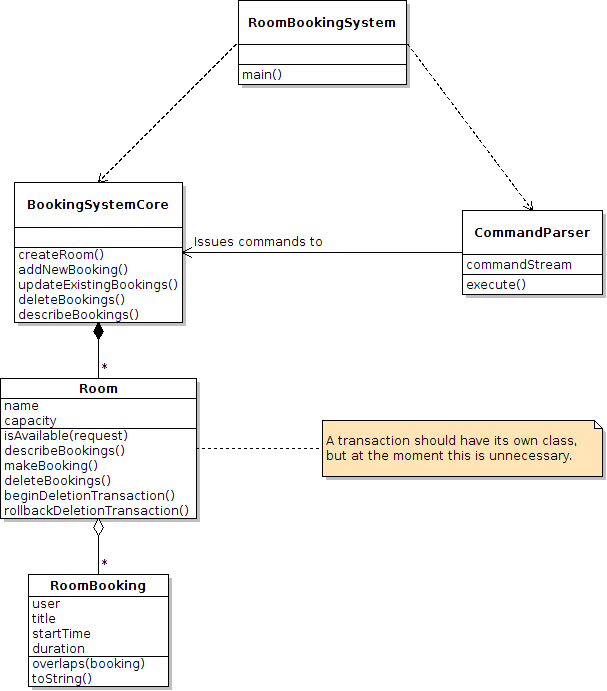
\includegraphics[scale=0.7]{../uml/RoomBooking.png}
\vspace{5mm}

\texttt{User} and \texttt{Transaction} classes have not been added to this
system, since otherwise they would be dumb wrappers around a \texttt{String} and
a \texttt{LinkedList}, respectively. They thus do not appear anywhere in this
diagram as separate entities. A \texttt{User} can be considered a property of
\texttt{RoomBooking}, and a \texttt{Transaction} is just an opaque object
that is internal to a \texttt{Room}.

While it may be argued that such approach is not sufficiently abstract, it leads
to more readable and simpler code. This is a deliberate trade-off.

\section*{Sequence diagram for the ``Change'' operation}

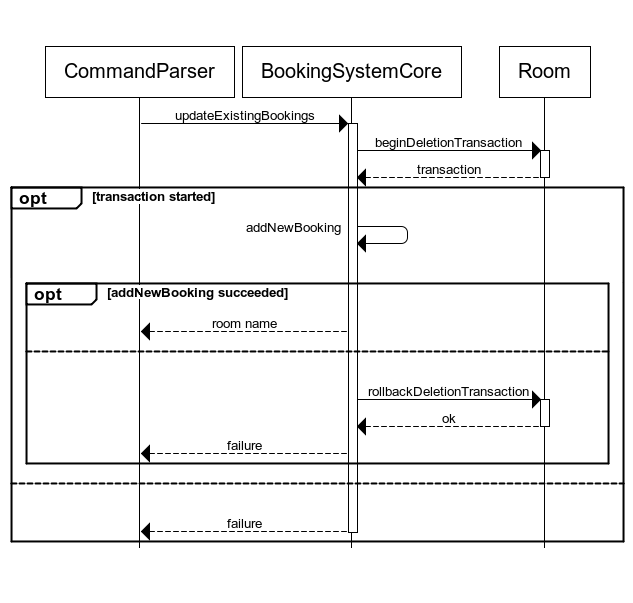
\includegraphics[scale=0.7]{../uml/sequence-bookings-change.png}

The simplest way to implement booking changes is to provide pseudo-transactions
to \texttt{BookingSystemCore}. As depicted above, we issue a deletion request to
the Room, and if that succeeds, we attempt to add a booking. If anything fails,
we abort and undo the deletion.

An alternative would be to check if the room we are deleting from contains the
requested bookings to be changed, and then if the new bookings can be added
without clashing with the ones not removed. That pushes most of the changing
procedure into \texttt{Room}'s logic, but makes it more convoluted.

Another alternative is to duplicate the entire set of bookings made to that
\texttt{Room} and reinstate it in case of failure, but that resembles the
current approach and is more wasteful.

\end{document}
